%Hoerkurven

\documentclass[tikz,convert={outfile=\jobname.png}]{standalone}
\input{../../tikzpic_packages.tex}

\begin{document}

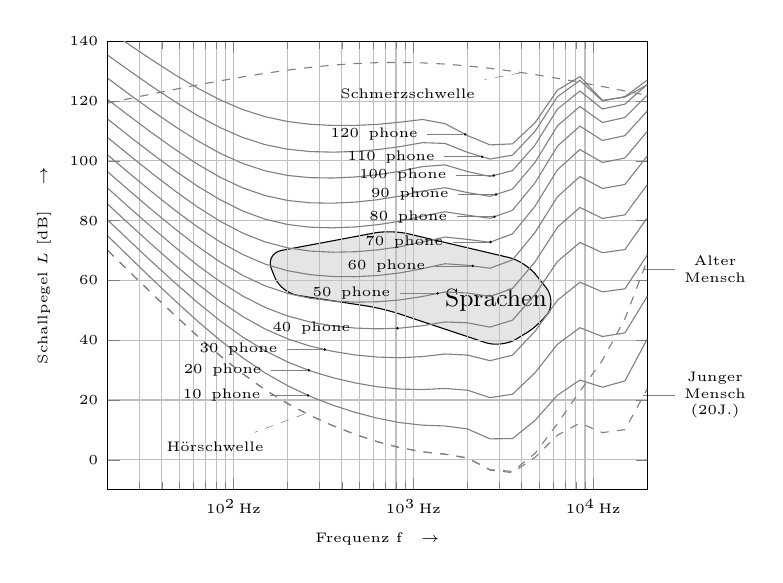
\begin{tikzpicture}
	\tikzset{font=\tiny,
	every node/.style={color=black}}
  \pgfplotsset{log base 10 number format code/.code={$10^{\pgfmathprintnumber{#1}}$\,Hz}}  
  
  
\draw[fill=gray!20,rounded corners=6pt] (2,3)--(2.2,2.5)--(3.5,2.3)--(5,1.8)--(5.5,2.1)--(5.7,2.4)node[left,font=\small]{Sprachen}--(5.3,2.9)--(3.6,3.3)--cycle;  
  
\draw[color=gray,very thin](6.8,2.8)--(7.2,2.8);
\node[style={font=\tiny},right,align=center] at (7.2,2.8){Alter \\ Mensch};

\draw[color=gray,very thin](6.8,1.2)--(7.2,1.2);
\node[style={font=\tiny},right,align=center] at (7.2,1.2){Junger \\ Mensch \\ (20J.)}; 
  
  \begin{semilogxaxis}[
    xmin=20, 
    xmax=20000, 
    domain=20:20000,
    grid=both,
    ymin=-10,
    ymax=140,
    ytick={0,20,...,140},
	xlabel={Frequenz f\quad $\rightarrow$},
	ylabel={Schallpegel $L$  \ensuremath{[}dB\ensuremath{]} \quad $\rightarrow$},
	clip=true   
    ]
   

\foreach \a in {1}{
	 \addplot[color=gray,mark=false,style=dashed,clip=false]{20*ln(
	 (2.5*10^6*(\a*10)*
	 ((x*\a/(1*10^3))^3+1)^(1/3)
	 *
	 ((x*\a/(1.5*10^2))^2+1)^(2/2)
	 *
	 ((x*\a/(3.5*10^3))^5+1)^(8/5)
	 *
	 ((x*\a/(1.35*10^4))^12+1)^(14/12)	 
	 )/(
	 (x*\a)^3
	 *
	 ((x*\a/(2.0*10^3))^12+1)^(3/12)
	 *
	 ((x*\a/(1.0*10^4))^4+1)^(14/4)))
	 /
	 (ln(10))} node[color=blue,pos=0.5,pin=210:{H\"orschwelle},inner sep=0pt]{};
}

\addplot[color=gray,mark=false,style=dashed,clip=false]{20*ln(
	 (2.5*10^6*(10)*
	 ((x/(1*10^3))^3+1)^(1/3)
	 *
	 ((x/(1.5*10^2))^2+1)^(2/2)
	 *
	 ((x/(3.5*10^3))^5+1)^(8/5)
	 *
	 ((x/(1.35*10^4))^12+1)^(5/12)	 
	 )/(
	 (x)^3
	 *
	 ((x/(2.0*10^3))^12+1)^(3/12)
	 *
	 ((x/(1.0*10^4))^4+1)^(2/4)))
	 /
	 (ln(10))};

\foreach \a in {10,20,30,...,120}{
	 \edef\temp{\noexpand\addplot[color=gray,mark=false,clip=true]{20*ln(
	 (3*10^7*10^(1.3*\a/80+\a^4/139^4)
	 *
	 ((x/(1*10^3))^3+1)^(1*((3/10-4/13)*\a+40/13)/3/3)
	 *
	 ((x/(1.5*10^2-\a/5))^2+1)^(2*(2-(1/65^2*(\a-67)^2))^(1/2)/2)
	 *
	 ((x/(3.5*10^3+\a*5))^5+1)^(8*(3/((3/10-4/13)*\a+40/13))^(0.9)/5)
	 *
	 ((x/(1.35*10^4-\a*12))^12+1)^(14/((3/10-4/13)*\a+40/13)*3/12)	 
	 )/(
	 (x)^((3/10-4/13)*\a+40/13)
	 *
	 ((x/(2.0*10^3-\a*80/14))^12+1)^(3/(2-(1/65^2*(\a-67)^2))^(1/2)/12)
	 *
	 ((x/(1.0*10^4))^4+1)^(14/((3/10-4/13)*\a+40/13)*((\a/8)^(1/6.5))*3/4)))
	 /
	 (ln(10))} node [pos=0.5,style={fill=black,circle},pin=180:{\a \, phone},inner sep=0pt] {};
	}
	\temp
	 
};

	\addplot[style=dashed,color=gray] {
	20*ln((13*10^4*x^(2/3))
	/
	((x/800)+1)^(4/3))
	/
	ln(10)} node [pos=0.7,pin=190:{Schmerzschwelle},inner sep=0pt] {};
    
  \end{semilogxaxis}


\end{tikzpicture}


\end{document}